\section{NP-Completude}

Nesta seção é demonstrado formalmente que o Problema do Caminho Hamiltoniano é NP-completo. Para isso, inicialmente mostra-se que o problema pertence à classe NP. Em seguida, é provado que o problema é NP-Completo por meio de reduções polinomiais, começando com uma redução do 3-SAT para o Problema do Caminho Hamiltoniano Dirigido que, por sua vez, é reduzido para não direcionado.

Antes de tudo, é necessário mostrar que Problema do Caminho Hamiltoniano (HAMPATH) pertence à classe NP. A instância é definida por um grafo não dirigido $G = (V, E)$ e o certificado por um caminho simples $P = (V', E')$, conforme definido anteriormente. A verificação de que $P$ é um caminho hamiltoniano em $G$ pode ser realizada em tempo polinomial da seguinte forma:

\begin{itemize}
    \item Verificar se $V' = V$, isto é, se $P$ e $G$ possuem os mesmos vértices.
    \item Para cada par consecutivo $v_i, v_{i+1}\in V'$, verificar se a aresta $v_iv_{i+1} \in E$.
\end{itemize}

Verificar se $V'=V$  pode ser feito em tempo $O(|V| \log |V| + |V'| \log |V'|)$, bastando ordenar $V$ e $V'$, e verificar se $|V|=|V'|$ e $\forall i= 1,\ldots,|V|$ se $v_i=v'_i$, com $v_i\in V$ e $v_i'\in V'$. Já a verificação da existência das arestas pode ser feita em tempo $O(|V|)$, iterando em $V'$ e assumindo que as arestas foram representadas como uma matiz/lista de adjacência. Logo, é possível verificar em tempo polinomial se um certificado $P$ é um caminho hamiltoniano em $G$ e portanto, HAMPATH pertence à classe NP.

Para provar que HAMPATH é NP-Completo, serão realizadas duas reduções: a primeira é do Problema da 3-Satisfatibilidade (3-SAT) (um problema NP-Completo \cite{Karp1972, cormen2012} bem conhecido) para o Problema do Caminho Hamiltoniano Dirigido (DHAMPATH), que por sua vez será reduzido para HAMPATH. De maneira análoga ao que foi provado anteriormente para HAMPATH, pode-se provar que DHAMPATH também pertence à classe NP.

\subsection{3-SAT \reduct DHAMPATH \texorpdfstring{\cite{Kleinberg2006}}{(Kleinberg; Tardos, 2006)}}

Seja uma instância arbitrária do 3-SAT com variáveis $x_1,\ldots,x_n$ e cláusulas $C_1,\ldots,C_k$. A fim de auxiliar a compreensão, será tomada como exemplo a seguinte expressão $E$ como instância do 3-SAT a ser reduzida: $$E=(x\lor\lnot y\lor z)\land(\lnot x\lor w\lor\lnot z)$$

A ideia é, a princípio, construir um grafo que contenha $2^n$ caminhos hamiltonianos possíveis, onde cada um deles representam as $2^n$ atribuições possíveis de valores às variáveis. Constrói-se $n$ caminhos $P_1, \ldots, P_n$ para cada variável, onde cada $P_i$ possui vértices $v_{i1}, v_{i2}, \ldots,v_{ib}$, onde $b>k$.

Uma variável pode estar em todas as $k$ cláusulas, então vamos assumir que $b=2k+2$, isto é, todo $P_i$ terá 2 vértices para cada cláusula e mais 2 extras (isso fará sentido adiante). Para cada vértice $v_{ij}$, com $1 \le j < b$, existem as arestas $v_{ij}v_{i,j+1}$ e $v_{i,j+1}v_{ij}$, ou seja, cada caminho $P_i$ pode ser percorrida da esquerda para a direita e vice-versa.

Os caminhos são conectados da seguinte forma: para cada $i=1,\ldots, n-1$, são criadas as arestas $v_{i1}v_{i+1,1}$, $v_{i1}v_{i+1,b}$, $v_{ib}v_{i+1,1}$ e $v_{ib}v_{i+1,b}$. São adicionados ao grafo 2 novos vértices $s$ e $t$ (para garantir que qualquer caminho hamiltoniano comece em $s$ e termine em $t$), e definidos as arestas $sv_{11}$, $sv_{1b}$, $tv_{n1}$ e $tv_{nb}$. Até este ponto, a estrutura do grafo está ilustrada abaixo na \reffig{fig:3-sat-para-chd_parcial}.

\begin{figure}[H]
    \centering
    \input{figuras/3-sat-para-chd_parcial}
    \caption{Grafo parcial formado da redução de 3-SAT para DHAMPATH}
    \label{fig:3-sat-para-chd_parcial}
\end{figure}

Seguindo o processo descrito anteriormente para $E$, com $n=4$ e $k=2$, são construídos 4 caminhos com $b=2\cdot2+2=6$ vértices cada. Adicionando os vértices $s$ e $t$, e conectando todos os vértices como já descrito, o grafo parcial para $E$ está ilustrado abaixo na \reffig{fig:3-sat-para-chd_parcial_exemplo}.

\begin{figure}[H]
    \centering
    \begin{tikzpicture}[
    node/.style={circle, draw, minimum size=6mm},
    >=Stealth
]

\def\xsep{3}
\def\ysep{1.75}

% ---------- Colunas ------------
\foreach \i [evaluate=\i as \yy using {-(\i-1)*\ysep}] in {1,...,6} {
  \node[node] (px\i) at (0,\yy) {$v_{x,\i}$};
  \node[node] (py\i) at (\xsep,\yy) {$v_{y,\i}$};
  \node[node] (pz\i) at (2*\xsep,\yy) {$v_{z,\i}$};
  \node[node] (pw\i) at (3*\xsep,\yy) {$v_{w,\i}$};
}

\foreach \i in {x,y,z,w} {
    \node at ($(p\i6)+(0,-1.2)$) {$P_\i$};
}

% ----------- Arestas internas -----------
\foreach \col in {px,py,pz,pw}{
  \foreach \i in {1,...,5}{
    \def\iinc{\the\numexpr\i+1\relax}
    \draw[->,bend left=15] (\col\i) to (\col\iinc);
    \draw[->,bend left=15] (\col\iinc) to (\col\i);
  }
}

% Vértices s e t
\path let \p1 = (px1), \p2 = (px6) in
  node[node] (s) at (-\xsep,{(\y1+\y2)/2}) {$s$};

\path let \p1 = (pw1), \p2 = (pw6) in
  node[node] (t) at (4*\xsep,{(\y1+\y2)/2}) {$t$};

\draw[->] (s) -- (px1);
\draw[->] (s) -- (px6);
\draw[->] (pw1) -- (t);
\draw[->] (pw6) -- (t);

% Conexões entre as colunas

\foreach \a/\b in {x/y,y/z,z/w} {
    \draw[->] (p\a1) -- (p\b1);
    \draw[->] (p\a1) -- (p\b6);
    \draw[->] (p\a6) -- (p\b1);
    \draw[->] (p\a6) -- (p\b6);
}

\end{tikzpicture}

    \caption{Grafo parcial formado da redução da instância $E$ do 3-SAT para DHAMPATH}
    \label{fig:3-sat-para-chd_parcial_exemplo}
\end{figure}

A ideia é que cada caminho hamiltoniano seja identificado da seguinte maneira: se o caminho percorrer $P_i$ da esquerda para direita, então $x_i$ é verdadeiro; caso contrário, é falso. Para modelar isso, serão adicionados novos $k$ vértices (um para cada cláusula) e a instância do 3-SAT será satisfatível se, e somente se, restar algum caminho hamiltoniano no grafo.

Seja $c_j$ o vértice da cláusula $C_j$. Para cada termo $t\in C_j$, se $t=x_i$, então adicionaremos as arestas $v_{i,2j}c_{j}$ e $c_{j}v_{i,2j+1}$; se $t=\lnot x_i$, então adicionaremos as arestas $v_{i,2j+1}c_{j}$ e $c_{j}v_{i,2j}$. A \reffig{fig:3-sat-para-chd_total} mostra visualmente como $c_j$ é adicionado ao grafo.

\begin{figure}[H]
    \centering
    \begin{tikzpicture}[
    node/.style={circle, draw, minimum size=6mm},
    dot/.style={inner sep=0pt},
    >=Stealth
]

    \def\xsep{3}
    \def\ysep{1.8}
    \def\xn{2.6*\xsep}
    \def\ycenter{-1.85*\ysep}
    
    % ---------- vértice s ----------
    \node[node] (s) at (-\xsep,\ycenter) {$s$};
    
    % ---------- Coluna P1 ----------
    \node[node] (p11) at (0,0) {$v_{1,1}$};
    \node[node] (p12) at (0,-\ysep) {$v_{1,2}$};
    \node[node] (p13) at (0,-2*\ysep) {$v_{1,3}$};
    \node at (0,-2.85*\ysep) {$\vdots$};
    \node[node] (p1k) at (0,-3.7*\ysep) {$v_{1,k}$};
    
    \node at ($(p1k)+(0,-1.2)$) {$P_1$};
    
    % ---------- Coluna P2 ----------
    \node[node] (p21) at (\xsep,0) {$v_{2,1}$};
    \node[node] (p22) at (\xsep,-\ysep) {$v_{2,2}$};
    \node[node] (p23) at (\xsep,-2*\ysep) {$v_{2,3}$};
    \node at (\xsep,-2.85*\ysep) {$\vdots$};
    \node[node] (p2k) at (\xsep,-3.7*\ysep) {$v_{2,k}$};
    
    \node at ($(p2k)+(0,-1.2)$) {$P_2$};
    
    % ---------- Reticências horizontais ----------
    \node (hdots) at ({(\xsep+\xn)/2}, -2*\ysep) {$\cdots$};
    
    % Pontos auxiliares para as arestas
    \node[dot] (L) at ($(hdots)+(-0.6,0)$) {};
    \node[dot] (R) at ($(hdots)+(0.6,0)$) {};
    
    % ---------- Coluna Pn ----------
    \node[node] (pn1) at (\xn,0) {$v_{n,1}$};
    \node[node] (pn2) at (\xn,-\ysep) {$v_{n,2}$};
    \node[node] (pn3) at (\xn,-2*\ysep) {$v_{n,3}$};
    \node at (\xn,-2.85*\ysep) {$\vdots$};
    \node[node] (pnk) at (\xn,-3.7*\ysep) {$v_{n,k}$};
    
    \node at ($(pnk)+(0,-1.2)$) {$P_n$};
    
    % ---------- vértice t ----------
    \node[node] (t) at (\xn+\xsep,\ycenter) {$t$};
    
    % ---------- Arestas internas ----------
    \foreach \a/\b in {p11/p12,p12/p13,p21/p22,p22/p23,pn1/pn2,pn2/pn3}{
      \draw[->,bend left=20] (\a) to (\b);
      \draw[->,bend left=20] (\b) to (\a);
    }
    
    % ---------- Arestas de P1 para P2 ----------
    \draw[->] (p11) -- (p21);
    \draw[->] (p11) -- (p2k);
    \draw[->] (p1k) -- (p21);
    \draw[->] (p1k) -- (p2k);
    
    % ---------- Adicionado manualmente ---------
    \def\edx{1.2}
    \def\eix{0.25}
    \def\eiy{0.55*\ysep}
    
    \draw[-] (p21) -- ++(\edx, 0);
    \draw[-] (p21) -- ++(\edx, -\ysep);
    \draw[-] (p2k) -- ++(\edx, 0);
    \draw[-] (p2k) -- ++(\edx, \ysep);
    
    \draw[<-] (pn1) -- ++(-\edx, 0);
    \draw[<-] (pn1) -- ++(-\edx, -\ysep);
    \draw[<-] (pnk) -- ++(-\edx, 0);
    \draw[<-] (pnk) -- ++(-\edx, \ysep);
    
    \node (hdotsTop) at ($(p21)!0.5!(pn1)$) {$\cdots$};
    \node (hdotsBottom) at ($(p2k)!0.5!(pnk)$) {$\cdots$};
    
    \foreach \a in {p13,p23,pn3}{
      \draw[-,bend left=10] (\a) to ++(\eix, -\eiy);
      \draw[<-,bend right=10] (\a) to ++(-\eix, -\eiy);
    }
    
    \foreach \a in {p1k,p2k,pnk}{
      \draw[<-,bend right=10] (\a) to ++(\eix, \eiy);
      \draw[-,bend left=10] (\a) to ++(-\eix, \eiy);
    }
    
    % ---------- Arestas com s e t ----------
    \draw[->] (s) -- (p11);
    \draw[->] (s) -- (p1k);
    \draw[->] (pn1) -- (t);
    \draw[->] (pnk) -- (t);
    
    % ------------- Vértice c1 ---------------
    \node[node] (c1) at ({0.5*\xsep}, {1.25*\ysep}) {$c_1$};
    
    \draw[->,dashed,out=45,in=225] (p12) to (c1);
    \draw[->,dashed,out=250,in=45] (c1) to (p13);
    
    \draw[->,dashed,out=300,in=135] (c1) to (p22);
    \draw[->,dashed,out=135,in=270] (p23) to (c1);
    
    \draw[->,dashed] (pn2) -- (c1);
    \draw[->,dashed] (c1) -- (pn3);


\end{tikzpicture}

    \caption{Grafo formado da redução de 3-SAT para DHAMPATH. Apenas o $c_1$ foi adicionado para uma melhor visualização, e as arestas que o ligam foram adicionadas sem perca de generalidade.}
    \label{fig:3-sat-para-chd_total}
\end{figure}

Tomando como exemplo a primeira cláusula de $E$ ($x\lor\lnot y\lor z$), o caminho hamiltoniano deve percorrer $P_x$ da esquerda para a direita, ou deve percorrer $P_y$ da direita para a esquerda, ou deve percorrer $P_z$ da esquerda para a direita. Então adiciona-se o vértice $c_1$ e as arestas $v_{x,2}c_1$, $c_1v_{x,3}$, $v_{y,3}c_1$, $c_1v_{y,2}$, $v_{z,2}c_1$, $c_1v_{z,3}$. De maneira análoga adiciona-se $c_2$ para a segunda cláusula de $E$ e suas respectivas arestas. A ilustração do grafo formado pela redução de $E$ para DHAMPATH está abaixo na \reffig{fig:3-sat-para-chd_total_exemplo} 

\begin{figure}[H]
    \centering
    \begin{tikzpicture}[
    node/.style={circle, draw, minimum size=6mm},
    >=Stealth
]

\def\xsep{3}
\def\ysep{1.75}

% ---------- Colunas ------------
\foreach \i [evaluate=\i as \yy using {-(\i-1)*\ysep}] in {1,...,6} {
  \node[node] (px\i) at (0,\yy) {$v_{x,\i}$};
  \node[node] (py\i) at (\xsep,\yy) {$v_{y,\i}$};
  \node[node] (pz\i) at (2*\xsep,\yy) {$v_{z,\i}$};
  \node[node] (pw\i) at (3*\xsep,\yy) {$v_{w,\i}$};
}

\foreach \i in {x,y,z,w} {
    \node at ($(p\i6)+(0,-1.2)$) {$P_\i$};
}

% ----------- c1 e c2 -----------
\node[node] (c1) at (0.5*\xsep,1.25*\ysep) {$c_1$};
\node[node] (c2) at (2.5*\xsep,1.25*\ysep) {$c_2$};

% ----------- Arestas internas -----------
\foreach \col in {px,py,pz,pw}{
  \foreach \i in {1,...,5}{
    \def\iinc{\the\numexpr\i+1\relax}
    \draw[->,bend left=15, red] (\col\i) to (\col\iinc);
    \draw[->,bend left=15] (\col\iinc) to (\col\i);
  }
}

\draw[->,bend left=15] (px2) to (px3);
\draw[->,bend left=15] (pw4) to (pw5);

% ----------- Conexões com c1 -----------
% Px
\draw[->,dashed,out=45,in=210,red] (px2) to (c1);
\draw[->,dashed,out=240,in=45,red] (c1) to (px3);

% Py (invertido)
\draw[->,dashed,out=300,in=135] (c1) to (py2);
\draw[->,dashed,out=135,in=270] (py3) to (c1);

% Pz
\draw[->,dashed] (pz2) -- (c1);
\draw[->,dashed] (c1) -- (pz3);

% ----------- Conexões com c2 -----------
% Px (invertido)
\draw[->,dashed,out=180,in=30] (c2) to (px4);
\draw[->,dashed,out=30,in=210] (px5) to (c2);

% Pz (invertido)
\draw[->,dashed,out=240,in=45] (c2) to (pz4);
\draw[->,dashed,out=30,in=270] (pz5) to (c2);

% Pw (normal)
\draw[->,dashed,out=30,in=0,red] (pw4) to (c2);
\draw[->,dashed,out=330,in=30,red] (c2) to (pw5);

% Vértices s e t
\path let \p1 = (px1), \p2 = (px6) in
  node[node] (s) at (-\xsep,{(\y1+\y2)/2}) {$s$};

\path let \p1 = (pw1), \p2 = (pw6) in
  node[node] (t) at (4*\xsep,{(\y1+\y2)/2}) {$t$};

\draw[->,red] (s) -- (px1);
\draw[->] (s) -- (px6);
\draw[->] (pw1) -- (t);
\draw[->,red] (pw6) -- (t);

% Conexões entre as colunas

\foreach \a/\b in {x/y,y/z,z/w} {
    \draw[->] (p\a1) -- (p\b1);
    \draw[->] (p\a1) -- (p\b6);
    \draw[->, red] (p\a6) -- (p\b1);
    \draw[->] (p\a6) -- (p\b6);
}

\end{tikzpicture}

    \caption{Grafo formado da redução da instância $E$ do 3-SAT para DHAMPATH. As arestas que formam um caminho hamiltoniano no grafo está destacado em vermelho, indicando que $E$ é satisfatível.}
    \label{fig:3-sat-para-chd_total_exemplo}
\end{figure}

Isso completa a construção do grafo e, consequentemente, a redução. O grafo possui $n$ caminhos $P_i$ de $b=2k+2$ vértices, $k$ vértices de cláusulas, um de início e outro final, totalizando $2nk+2n+k+2 = \Theta(nk)$ vértices. Em cada caminho $P_i$, há 2 arestas entre dois vértices adjacentes (ida e volta), e mais 2 em $v_{i1}$ e $v_{i,b}$ para conexão com $P_{i+1}$ (com exceção de $P_n$), além de mais 2 conectando $s$ com $P_1$ e 2 conectando $P_n$ com $t$, e mais 6 para cada $c_j$, totalizando $4nk+6n+6k=\Theta(nk)$ arestas. Considerando que a criação dos vértices quanto das arestas são realizadas em tempo $\Theta(nk)$ para ambos, pode-se afirmar que a redução é polinomial.

Agora será provado que uma instância do 3-SAT é satisfatível se, e somente se, o grafo construído a partir da redução possuir um caminho hamiltoniano. Dado uma instância $I=(\{x_1,\ldots,x_n\},;\{C_1,\ldots,C_k\})$ qualquer do 3-SAT, supõe-se que exista uma atribuição das variáveis que a satisfaça. Se $x_i$ for verdadeiro, espera-se que $P_i$ seja ``percorrido'' da esquerda para a direita; caso contrário, da direita para a esquerda. Para cada $C_j$, como ela é satisfeita pela atribuição, haverá ao menos um caminho $P_i$ que será percorrido na direção ``correta'' em relação à $c_j$, e podemos inseri-lo no percurso por meio das arestas incidentes em $v_{i,2j}$ e $v_{i,2j+1}$.

Por outro lado, supõe-se que exista um caminho hamiltoniano $P$ no grafo. Se $P$ entra em um vértice $c_j$ por uma aresta proveniente de $v_{i,2j}$, ele deve sair por uma aresta para $v_{i,2j+1}$. Caso contrário, $v_{i,2j+1}$ terá apenas um vizinho não visitado restante, ou seja, $v_{i,2j+2}$ e, portanto, o percurso não poderá visitar esse vértice e ainda manter a propriedade hamiltoniana. Simetricamente, se entra por $v_{i,2j+1}$ deve-se sair por $v_{i,2j}$.

Os vértices imediatamente anteriores e posteriores a $c_j$ no caminho $P$ são unidos por uma aresta $e$ no grafo; portanto, se $c_j$ for removido do caminho e for inserido $e$ cada $j$, obtém-se um caminho hamiltoniano $P'$ no subgrafo formado ao remover $c_1,\ldots,c_k$ (grafo original, antes dos vértices de cláusula serem adicionados). Qualquer caminho hamiltoniano neste subgrafo deve percorrer cada $P_i$ completamente em uma direção ou outra.

Assim, $P'$ é usado para definir a seguinte atribuição de verdade para a instância do 3-SAT: Se $P'$ percorrer $P_i$ da esquerda para a direita, $x_i = 1$; caso contrário, $xi = 0$. Como o caminho maior $P$ foi capaz de visitar cada vértice de cláusula $c_j$, pelo menos um dos caminhos foi percorrido na direção “correta” em
relação ao vértice $c_j$, e, portanto, a atribuição definida até aqui satisfaz todas as cláusulas. 

Tendo estabelecido que a instância do 3-SAT é satisfatível se, e somente se, o grafo possuir um caminho hamiltoniano, portanto, DHAMPATH é NP-Completo.


\subsection{DHAMPATH \reduct HAMPATH}

Seja $G=(V,E)$ um grafo dirigido qualquer. A fim de auxiliar a compreensão, será tomado como exemplo o seguinte grafo como instância do DHAMPATH a ser reduzida para HAMPATH:

\begin{figure}[H]
    \centering
    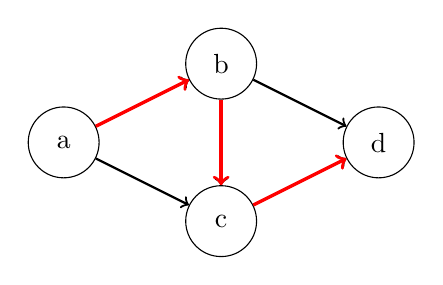
\begin{tikzpicture}[
    vertex/.style={circle, draw, minimum size=9mm, inner sep=0pt},
    edge/.style={->, thick},
    pathedge/.style={->, very thick, red}
]

    \node[vertex] (a) at (0,1.5) {a};
    \node[vertex] (b) at (2,2.5) {b};
    \node[vertex] (c) at (2,0.5) {c};
    \node[vertex] (d) at (4,1.5) {d};
    
    % Arestas do grafo
    \draw[edge] (a) -- (b);
    \draw[edge] (a) -- (c);
    \draw[edge] (b) -- (c);
    \draw[edge] (b) -- (d);
    \draw[edge] (c) -- (d);
    
    % Caminho destacado a -> b -> c -> d
    \draw[pathedge] (a) -- (b);
    \draw[pathedge] (b) -- (c);
    \draw[pathedge] (c) -- (d);

\end{tikzpicture}
    \caption{Grafo dirigido a ser reduzido para não dirigido. As arestas em vermelho destacam o caminho hamiltoniano do grafo.}
    \label{fig:chd-para-chnd_grafo_exemplo}
\end{figure}

\noindent A ideia é transformar cada vértice de G em uma pequena subestrutura que force o caminho a ter uma direção lógica, ainda que as arestas não tenham direção no novo grafo $G'$.

Para cada vértice $v\in V$, são criados 3 vértices em $G'$: $v_{in}$ (entrada), $v_{mid}$ (meio) e $v_{out}$ (saída). Depois são adicionadas as seguintes arestas em $G'$: $v_{in}v_{mid}$ e $v_{mid}v_{out}$. Após isso, para cada vértice $uv\in E$ é adicionado a aresta $u_{out}v_{in}$. A \reffig{fig:chd-para-chnd_grafo_reduzido} ilustra como o grafo de exemplo ficou após esses processos.

\begin{figure}[H]
    \centering
    \begin{tikzpicture}[
    vertex/.style={circle, draw, minimum size=9mm, inner sep=0pt},
    edge/.style={-, thick},
    pathedge/.style={-, very thick, red}
]

    % Posições globais do diamante
    \node (A) at (-2,1.5) {};
    \node (B) at (2,2.75) {};
    \node (C) at (2,0.25) {};
    \node (D) at (6,1.5) {};
    
    % Deslocamento interno maior
    \def\d{1.5}
    
    % a_in, a_mid, a_out
    \node[vertex] (ain)  at ($(A)+(-\d,0)$) {$a_{in}$};
    \node[vertex] (amid) at (A)            {$a_{mid}$};
    \node[vertex] (aout) at ($(A)+(\d,0)$)  {$a_{out}$};
    
    % b_in, b_mid, b_out
    \node[vertex] (bin)  at ($(B)+(-\d,0)$) {$b_{in}$};
    \node[vertex] (bmid) at (B)            {$b_{mid}$};
    \node[vertex] (bout) at ($(B)+(\d,0)$)  {$b_{out}$};
    
    % c_in, c_mid, c_out
    \node[vertex] (cin)  at ($(C)+(-\d,0)$) {$c_{in}$};
    \node[vertex] (cmid) at (C)            {$c_{mid}$};
    \node[vertex] (cout) at ($(C)+(\d,0)$)  {$c_{out}$};
    
    % d_in, d_mid, d_out
    \node[vertex] (din)  at ($(D)+(-\d,0)$) {$d_{in}$};
    \node[vertex] (dmid) at (D)            {$d_{mid}$};
    \node[vertex] (dout) at ($(D)+(\d,0)$)  {$d_{out}$};
    
    % Arestas internas
    \draw[edge] (ain) -- (amid) -- (aout);
    \draw[edge] (bin) -- (bmid) -- (bout);
    \draw[edge] (cin) -- (cmid) -- (cout);
    \draw[edge] (din) -- (dmid) -- (dout);
    
    % Arestas conforme o grafo original
    \draw[edge] (aout) -- (bin);
    \draw[edge] (aout) -- (cin);
    \draw[edge] (bout) -- (cin);
    \draw[edge] (bout) -- (din);
    \draw[edge] (cout) -- (din);
    
    % Caminho destacado
    \draw[pathedge] (ain) -- (amid) -- (aout) -- (bin) -- (bmid) -- (bout)
                   -- (cin) -- (cmid) -- (cout) -- (din) -- (dmid) -- (dout);

\end{tikzpicture}

    \caption{Grafo dirigido reduzido para não dirigido. As arestas em vermelho destacam o caminho hamiltoniano do grafo.}
    \label{fig:chd-para-chnd_grafo_reduzido}
\end{figure}

Com isso, a redução do DHAMPATH para HAMPATH está concluída. Em $G$ O número de vértices é $3|V|=\Theta(|V|)$, enquanto o número de arestas é $2|V|+|E|=\Theta(|V|+|E|)$ (2 arestas internas por vértice mais as arestas originais). Considerando que a construção dos vértices e arestas em $G'$ são realizadas em tempo $\Theta(|V|)+\Theta(|V|+|E|)=\Theta(|V|+|E|)$, pode-se afirmar que a redução é polinomial.

Agora será provado que $G$ possui um caminho hamiltoniano se, e somente se, $G'$ possui um caminho hamiltoniano. Supondo que exista um caminho hamiltoniano em $G$, ele pode ser organizado em uma sequência de vértices $v_1,v_2,\ldots,v_n$, onde $\forall i=1,\ldots,n-1,\;v_iv_{i+1}\in E$. A partir dessa sequência, pode-se construir a sequência $v_{1}^{in},v_{1}^{mid},v_{1}^{out},v_{2}^{in},v_{2}^{mid},v_{2}^{out},\ldots,v_{n}^{in},v_{n}^{mid},v_{n}^{out}$, onde cada 2 vértices adjacentes são ligados por uma aresta. As arestas $v_{i}^{in}v_{i}^{mid}$ e $v_{i}^{mid}v_{i}^{out}$ existem por construção, enquanto $v_{i}^{out},v_{i+1}^{in}$ existe porque $v_iv_{i+1}\in E$. Logo, Esse caminho cobre todos os $3n$ vértices uma única vez.

Por outro lado, supondo que exista um caminho hamiltoniano em $G'$, em cada vértice $v\in V$ o seu representante $v_{mid}$ está conectado apenas à $v_{in}$ e $v_{out}$; logo, qualquer caminho hamiltoniano que visite $v_{mid}$ deve entrar por um vizinho e sair imediatamente pelo outro, ou seja, $v_{in},v_{mid}$ e $v_{out}$ devem ser percorridos consecutivamente. A única forma de conectar um bloco $\{u_{in},u_{mid},u_{out}\}$ a outro bloco $\{v_{in},v_{mid},v_{out}\}$ é através de uma aresta $u_{out}v_{in}$ ou $v_{in},u_{out}$, que por sua vez, por construção, só existem se houver uma aresta $uv$ ou $vu$, respectivamente, em $G$. Portanto, a sequência de blocos visitados em $G'$ corresponde diretamente à sequência de vértices em $G$.

Tendo estabelecido que a instância do DHAMPATH possui um caminho hamiltoniano se, e somente se, a sua redução para HAMPATH também possuir um caminho hamiltoniano, portanto, HAMPATH é NP-Completo.